\chapter{Dialogue Systems} \label{chap:dialogue_systems}

%Two basic transfer functions are shown in \cref{fig:methods:transfer_functions}. \label{chap:modules}

%\begin{figure}[H]
%  \centering
%  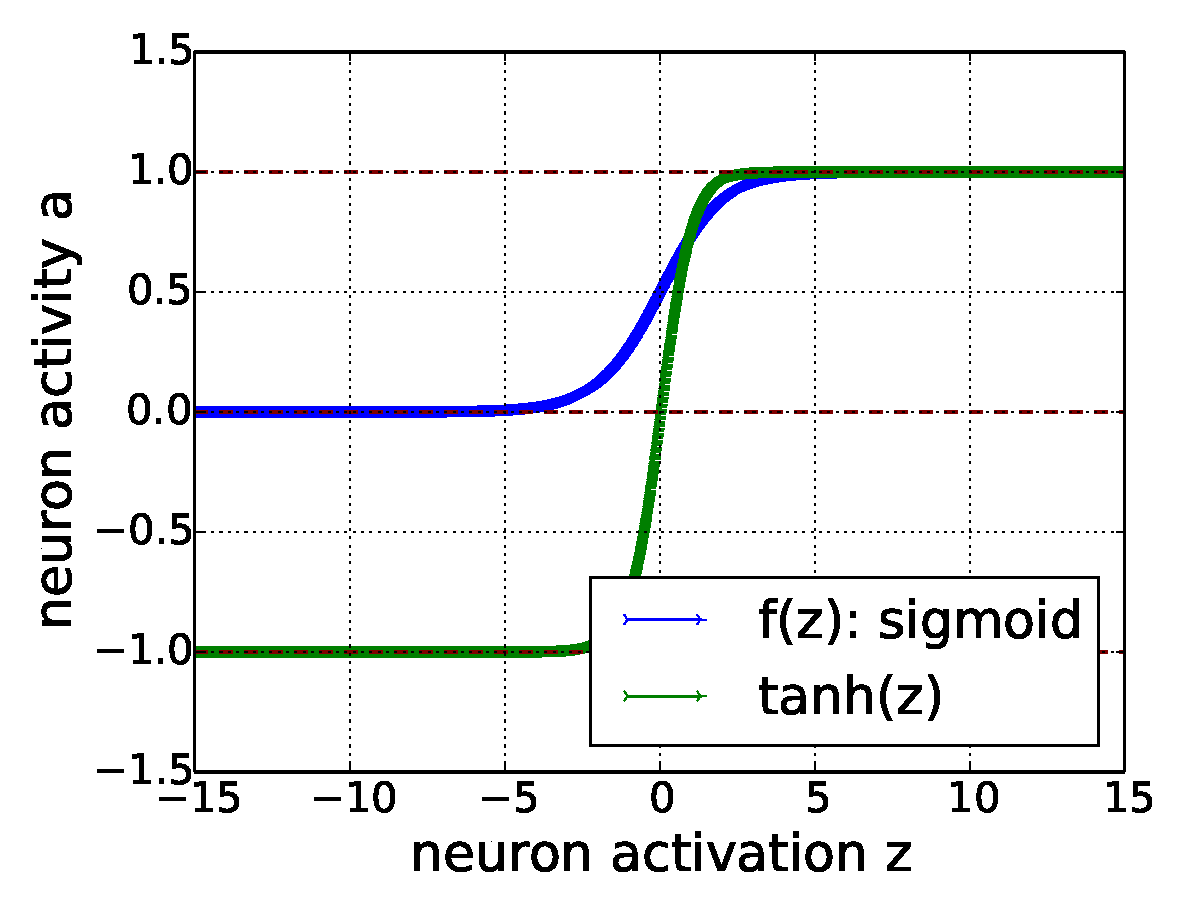
\includegraphics[width=0.7\textwidth]{transfer_functions.eps}
%  \caption{Transfer functions: \textit{Sigmoid} and \textit{Tanh}}
%  \label{fig:methods:transfer_functions}
%\end{figure}

\section{Automatic Speech Recognition}

Automatic Speech Recognition (ASR) is a way of converting sound into text.

Sound is nothing more than vibrations of the air that we humans are trained exceptionally well to decode. Moreover, now, we are teaching our computers how to do this. In the beginning, we have a stream of words that a person has uttered. The sound is picked up by a microphone and converted to a digital signal through a sound card, which means a stream of ones and zeroes.

One of the possible approaches in ASR modelling is, for example, at the level of phonemes or the level of whole words. We will only give an example here at the phoneme level, as the other approaches are very similar.

The first step the ASR system do is process the sound. It steps the sound to have chunks of speech that can be worked with and that can be mapped to letters. These chunks are called phones.

% The first step the ASR system do is process the sound. It steps the sound to have chunks of speech (shown in \cref{fig:chunked_voice}) that can be worked with and that can be mapped to letters. These chunks are called phones.

% \begin{figure}[H]
%     \centering
%     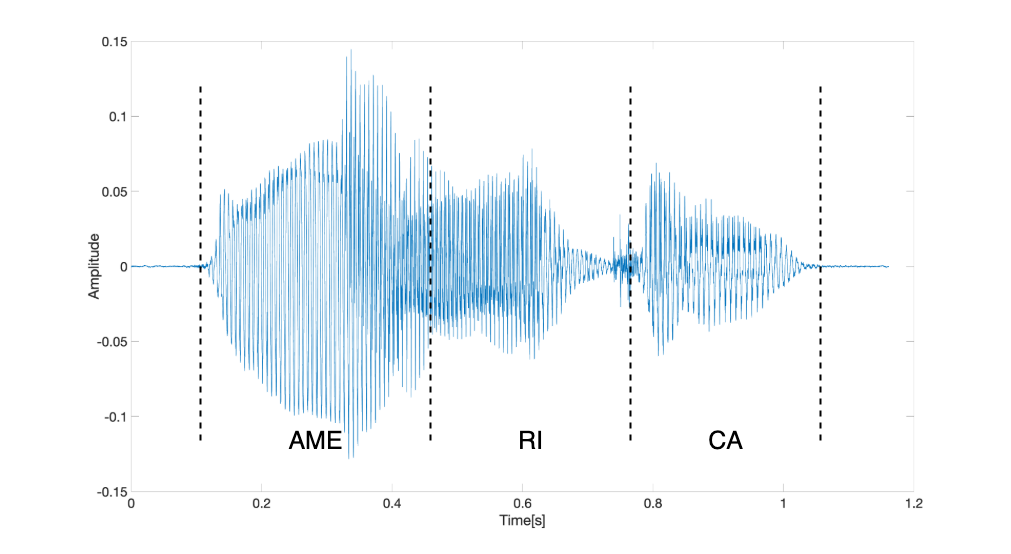
\includegraphics[width=\textwidth]{img/voice_edit.png}
%     \caption{Chunked speech signal}
%     \label{fig:chunked_voice}
% \end{figure}

The part of ASR responsible for mapping sound to phones is called the \textit{acoustic model} as a set of building blocks, boxes which contain models for all phones in a given language as showing in \cref{fig:phones_boxes}.

\begin{figure}[H]
    \centering
    
\includegraphics[width=0.7\textwidth]{img/phones_boxes.png}
    \caption{Phones boxes}
    \label{fig:phones_boxes}
\end{figure}

There are boxes labelled, for example, A, B, C, depending on which phones are used in the particular language. On top of that, part of this construction set is also contextual probabilities. It means how likely a phone is to follow another. The acoustic model's task is to guess which phones have been pronounced and how they combine into a word. The acoustic model processes the sound and compares it to the models of individual phones from its boxes. Since speech is very complex in a real scenario, the chunks that a person uttered will be similar to more than one box. The acoustic model takes this into account and also looks at the neighbouring chunks and their contextual probabilities. For example, in the string "HELLO", the second phoneme that a person uttered might have been E. However, it also could have been \begin{IPA}@\end{IPA}, A or even I, with different degrees of certainty. The next phoneme is probably L, but it also could be R. There are different probabilities of these phones in context, for example, H followed by E is more likely, at least in English, than H followed by I. The ASR system combines these bits of information and outputs the most likely result - a string of phones.\citep{stanislav_petr_2020}

The next step is to convert it into words. Nevertheless, this part can be tricky because the ASR does not know when a word starts or ends. Contrary to popular belief, there are no pauses between words in fluent speech. This particular string "heloumaj..." of phones can constitute several different phrases, for example, "hell oh my nay miss" or "hello mine aim is", or "hello my name is". The part of ASR responsible for mapping phones to words and phrases is called the language model.

Hidden Markov Models (HMM) are widely used for the statistical approach for automatic speech recognition. Suppose that \linebreak$W=\left\{w_{1}, w_{2}, \ldots, w_{N}\right\}$ is a sequence of words, and $O=\left\{o_{1}, o_{2}, \ldots, o_{N}\right\}$ is a sequence of phones. These sequences are taken with a period of 10 ms for segments of speech of length from 20 to 40 ms. The Bayes Theorem for conditional probability is used to figure out which phones have been pronounced and how they combine into a word.

\begin{equation}
    \boldsymbol{W}^{\prime}=\underset{w}{\operatorname{argmax}} P(\boldsymbol{W} \mid \boldsymbol{O})=\underset{w}{\operatorname{argmax}} \frac{P(\boldsymbol{W}) P(\boldsymbol{O} \mid \boldsymbol{W})}{P(\boldsymbol{O})}
\end{equation}




where P(W) is the a priori probability of word W, P(O|W) is the probability that the sequence of phones O will be generated under the conditions of pronouncing the sequence of words W, P(O) is the a priori probability of the sequence of phones O. 

Since the probability P(O) is independent of the sequence of words W, it is possible to modify the equation into the form shown in \cref{fig:bayes}:

% \begin{equation}
%     \boldsymbol{W}^{\prime}=\underset{w}{\operatorname{argmax}} P(\boldsymbol{W} \mid \boldsymbol{O})=\underset{w}{\operatorname{argmax}} P(\boldsymbol{W}) P(\boldsymbol{O} \mid \boldsymbol{W})
% \end{equation}

\begin{figure}[H]
	\centering
	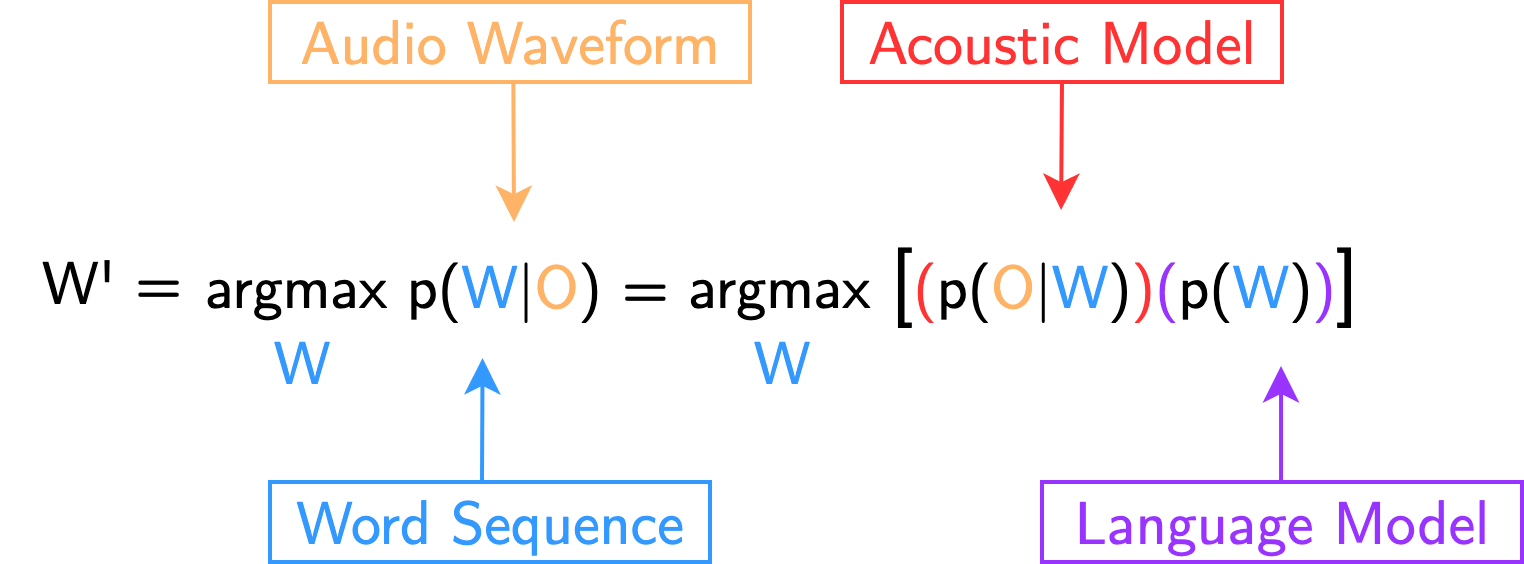
\includegraphics[width=\textwidth]{img/asr_bayes.png}
	\caption{The relation among acoustic model, language model and Bayes theorem}
	\label{fig:bayes}
\end{figure}

Nowadays, HMM is no longer used much, and Neural Networks techniques have become more common.

\section{Automatic Speech Synthesis}

The task of generating a speech out of text information has originally two approaches:
\begin{enumerate}
    \item concatenative (unit selection);
    \item statistical parametric.
\end{enumerate}

The concatenative synthesis is based on sequential combining of shot prerecorded samples of the speech. These samples can be stored in a database as of whole sentences, phrases, words and different phonemes. It depends on the application of the solutions. Building the unit selections synthesis model consists of three steps:

\begin{enumerate}
    \item Recording of the whole selected speech units in no possible context.
    \item Labelling segmentation of units.
    \item Choosing the most appropriate units. 
\end{enumerate}

The concatenative method is the most straightforward approach to the speech generation. Disadvantages include the requirement to have an ample storage for recorded units and an inability to apply various changes to a voice.

The statistical parametric synthesis consists of two parts, as shown in \cref{fig:synthesis_model}. The training step's approach is to extract excitation parameters like fundamental frequency and dynamic features, and spectral parameters from the speech database. Then we estimate them using one of the statistical models. The Hidden Markov Model (HMM) is the most widely used for this task. It should be noted that HMM is conscious dependent. It means that in this step, in addition to phonetic context, linguistic and prosodic context is taken into account. In the synthesis part, at first given sentence is converted into points with a dependent label sequence, and then their chance HMM is constructed according to this sequence. Next, spectrum and excitation parameters are generated from the utterance HMM, and finally, speech waveforms are synthesized from these parameters using excitation generation and the speech synthesis filter. The advantages of the statistical parametric approach are:
\begin{enumerate}
    \item Small footprint
    \item No need to store the speech waveforms, only statistics language independence.
    \item Flexibility in changing voice characteristics speaking styles and emotions.
\end{enumerate}
The most noticeable drawback is the quality of a synthesized speech.

\begin{figure}[H]
    \centering
    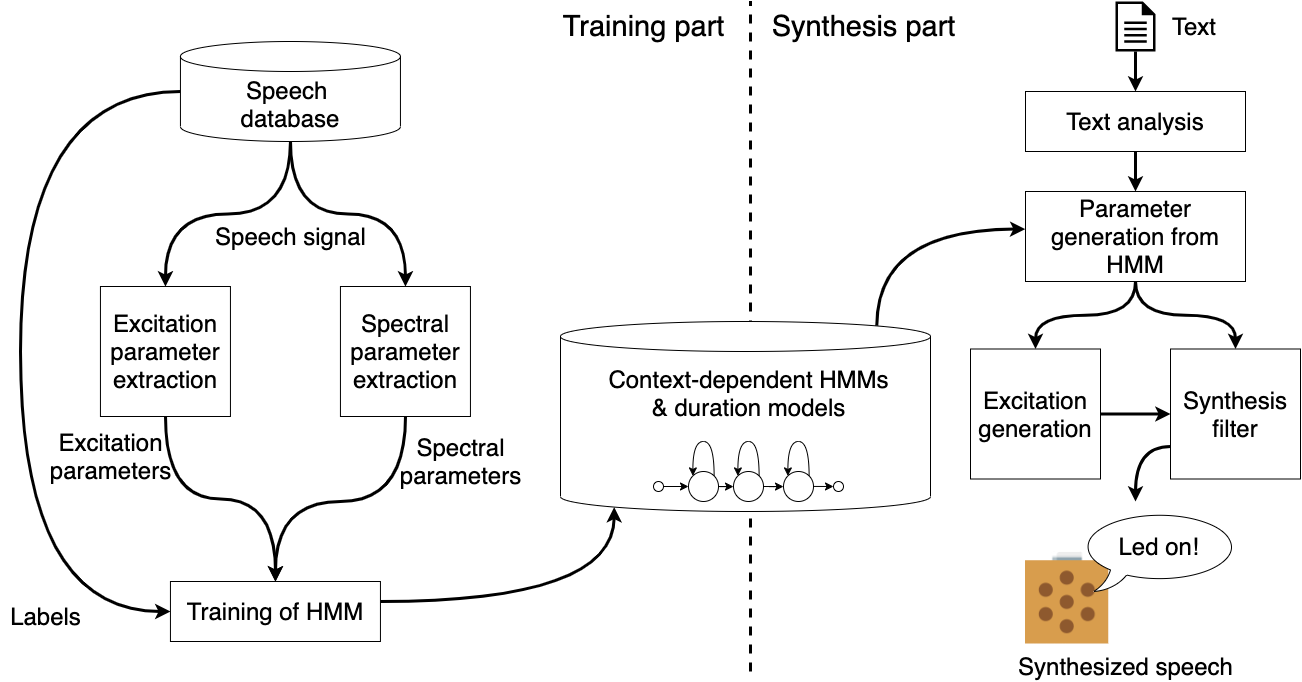
\includegraphics[width=\textwidth]{img/synthesis_model.png}
    \caption{Statistical parametric speech synthesis \citep{statistical_parametric_speech_synthesis_ZEN20091039}}
    \label{fig:synthesis_model}
\end{figure}

Procedures have changed over time, and Neural Networks (NN) and Long-Term Memory (TSLM) techniques have become more common in statistical parametric synthesis.

\section{The SpeechCloud Platform}

The SpeechCloud platform, developed at the Department of Cybernetics of the University of West Bohemia, is a system that connects ASR and TTS systems operating together via one interface. It is then possible to use these systems by many applications simultaneously through this interface. An independent instance is created for each dialogue system, allowing a client to create a characteristic language model, send a speech record to recognize, and receive the synthesized speech.

SpeechCloud provides the same services to all clients unless limited or specified otherwise. Each client should have the same functions, but each device, experiment or project is separated from the others, so the results are not affected by the unwanted intervention.

The architecture of the SpeechCloud and the connection to the client is briefly visualized in \cref{fig:speechcloud_schema}. The SpeechCloud using the module SCAPIServer as a primary point to establish a connection with the client application. Thus, the module negotiates with the client a specific application configuration, a control communication channel and the authentication of the session. The SCAPIServer then provides these pieces of information to other modules. The SIPSwitch module mediates the audio data transfer service between the SCWorker component and the client application. One instance of the SCWorker component is reserved for each client that holds one ASR and TTS instance. The SCWorker component has access to a TCP/IP network connection to collect additional data sources.

\begin{figure}[H]
    \centering
    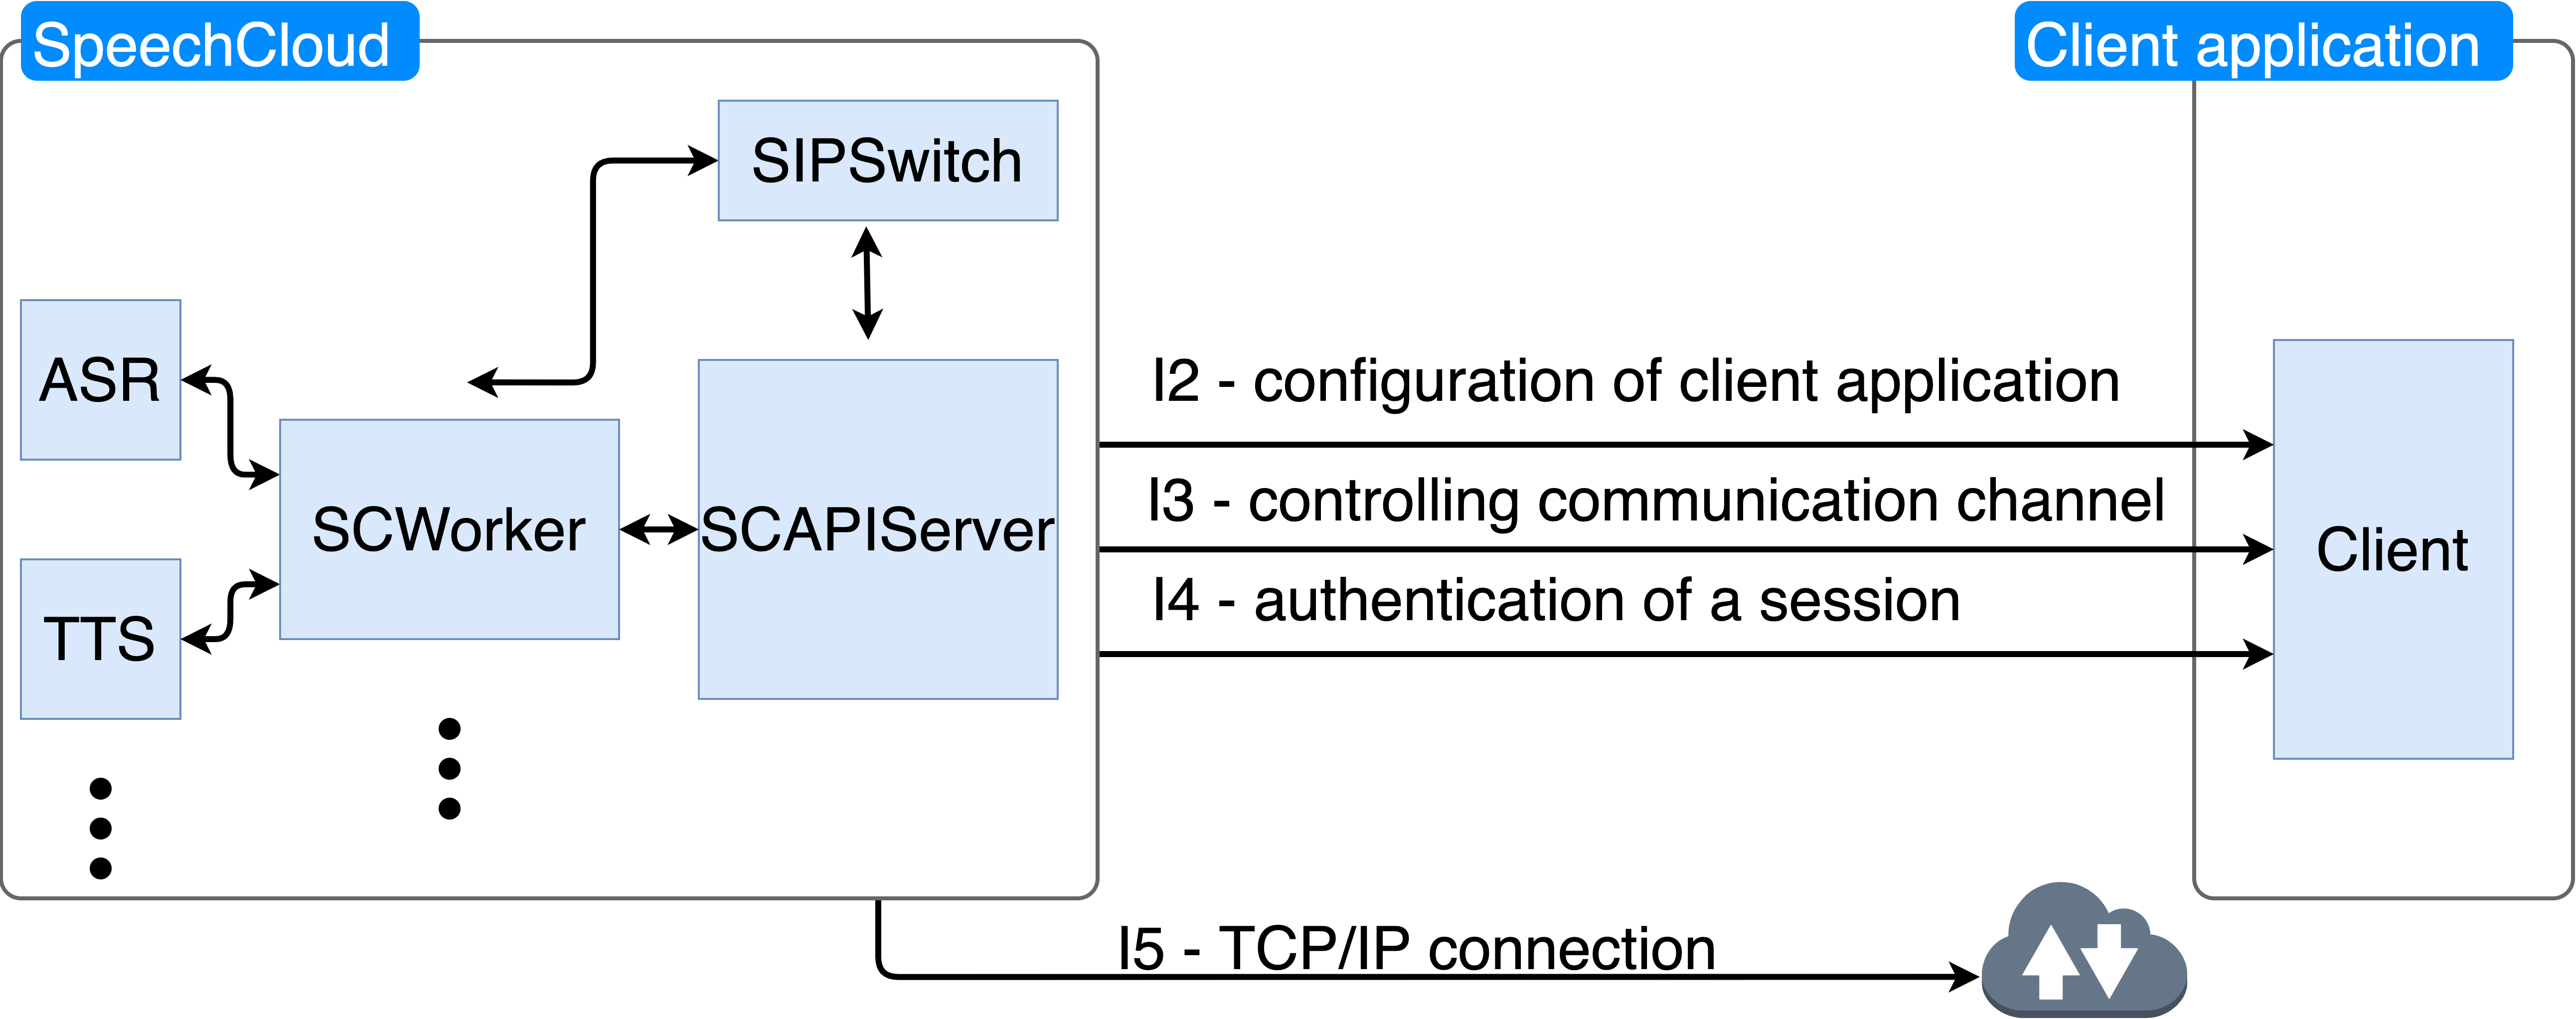
\includegraphics[width=\textwidth]{img/speechcloud_schema.png}
    \caption{SpeechCloud schema}
    \label{fig:speechcloud_schema}
\end{figure}

Solving the subject of the connection and transmission of data to the SpeechCloud via Internet communication protocols is not the content of this work hence are used ready-made software components and the SpeechCloud platform is used as a service.